\section{Results}
\label{sec:results}

Across the ten datasets, three seeds, four imbalance ratios, and five
contamination rates (the shared clean condition plus four noise levels in
each of the two directions), the full matrix produced 12{,}837 per-seed runs
over the nine methods (seven corrections plus the two uncorrected
baselines), seed-averaged into 4{,}279 method-condition rows. Of these,
123 runs failed outright, all \texttt{tabpfn\_downsample} at $r{=}0.50$
(Section~\ref{sec:methods-corrections}). 120 failed under Direction A
contamination, at every dataset, every nonzero $c$, and every seed, and 3
failed in the shared clean condition. Because the Direction A failures are
complete rather than sporadic, every $r{=}0.50$ block is entirely absent for
\texttt{tabpfn\_downsample} under Direction A, which is why the TabPFN
family's Direction A significance test below runs on 120 blocks rather than
160 (Section~\ref{sec:results-significance}). All other results below are
computed only over runs that completed.

\subsection{Overall Correction Robustness}
\label{sec:results-rq1}

Every one of the seven correction methods produced at least one stress cell
with negative Correction Gain, confirming the pattern anticipated in
Section~\ref{sec:introduction}. No correction remains uniformly beneficial
once label error is present. How often this happens varies sharply by
method. Table~\ref{tab:robustness} summarizes Correction Harm Rate (CHR) and
mean Correction Gain (CG, on balanced accuracy) for every method in each
direction. \texttt{tabpfn\_threshold} is the most robust method by both
measures in both directions. Its CHR is 8.1\% under Direction A and 1.6\%
under Direction B, roughly five times below the next-lowest correction under
Direction B, and its mean CG (0.061 and 0.085) is the highest of any method
in both directions. \texttt{tabpfn\_distpfn} sits at the other end, with
the lowest mean CG under Direction A (0.016) and, together with
\texttt{tabpfn\_distpfn\_t}, the highest CHR in both directions (23.4\% and
31.9\% for \texttt{tabpfn\_distpfn}, 24.4\% and 30.9\% for
\texttt{tabpfn\_distpfn\_t}).

\begin{table}[t]
\centering
\caption{Correction Harm Rate and mean Correction Gain (balanced accuracy)
by method and direction, over noisy stress cells only ($c>0$).}
\label{tab:robustness}
\begin{tabular}{@{}lrrrr@{}}
\toprule
& \multicolumn{2}{c}{CHR} & \multicolumn{2}{c}{mean CG} \\
Method & Dir.\ A & Dir.\ B & Dir.\ A & Dir.\ B \\
\midrule
\texttt{xgb\_weighted}      & 0.169 & 0.094 & 0.020 & 0.029 \\
\texttt{xgb\_ros}           & 0.188 & 0.125 & 0.018 & 0.030 \\
\texttt{xgb\_smote}         & 0.213 & 0.081 & 0.024 & 0.040 \\
\texttt{tabpfn\_threshold}  & 0.081 & 0.016 & 0.061 & 0.085 \\
\texttt{tabpfn\_distpfn}    & 0.234 & 0.319 & 0.016 & 0.010 \\
\texttt{tabpfn\_distpfn\_t} & 0.244 & 0.309 & 0.021 & 0.015 \\
\texttt{tabpfn\_downsample} & 0.217 & 0.075 & 0.051 & 0.071 \\
\bottomrule
\end{tabular}
\end{table}

Figure~\ref{fig:gain-heatmap} makes the same contrast spatially, comparing
\texttt{tabpfn\_threshold} (top row) against \texttt{tabpfn\_distpfn}
(bottom row) across every tested combination of imbalance ratio $r$ and
noise level $c$. \texttt{tabpfn\_threshold}'s gain stays positive across the
entire grid in both directions. \texttt{tabpfn\_distpfn}'s harm is not
spread evenly. It concentrates specifically at $r{=}0.50$ (near-balanced
classes) combined with the highest tested contamination, $c{=}0.30$, where
the correction actively hurts balanced accuracy rather than merely failing
to help.

\begin{figure*}[t]
\centering
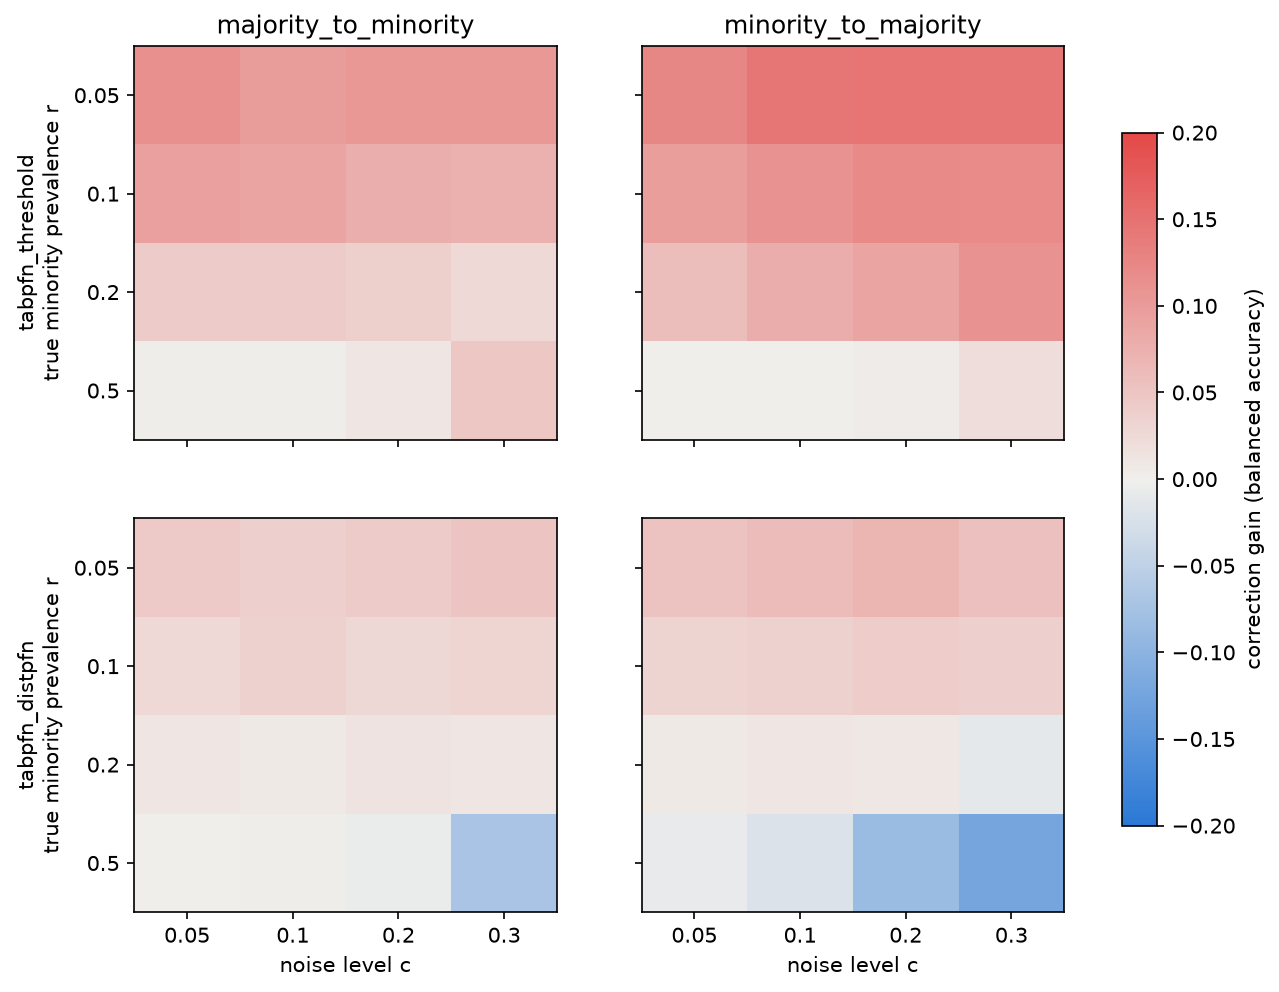
\includegraphics[width=0.85\linewidth]{figures/gain_heatmap_pair.png}
\caption{Correction gain (balanced accuracy) across imbalance ratio $r$ and
noise level $c$, for the most robust corrected method
(\texttt{tabpfn\_threshold}, top) and the least robust
(\texttt{tabpfn\_distpfn}, bottom). Blue indicates the correction hurt
relative to the uncorrected baseline at that cell, and red indicates it
helped.}
\label{fig:gain-heatmap}
\end{figure*}

\subsection{Direction-Dependent Failure}
\label{sec:results-rq2}

Corruption direction changes how often a correction fails, and the
direction of the effect is itself method-dependent rather than uniform.
Five of the seven methods have a higher CHR under Direction A
(majority rows relabeled as minority) than under Direction B (minority rows
relabeled as majority). These are \texttt{xgb\_ros}, \texttt{xgb\_smote},
\texttt{xgb\_weighted}, \texttt{tabpfn\_downsample}, and
\texttt{tabpfn\_threshold}, the last two by a wide margin
(Table~\ref{tab:robustness}). The two DistPFN variants show the opposite
pattern, failing more often under Direction B than Direction A.
Figure~\ref{fig:chr-regret} shows CHR and mean regret side by side for
every method, split by direction.

\begin{figure*}[t]
\centering
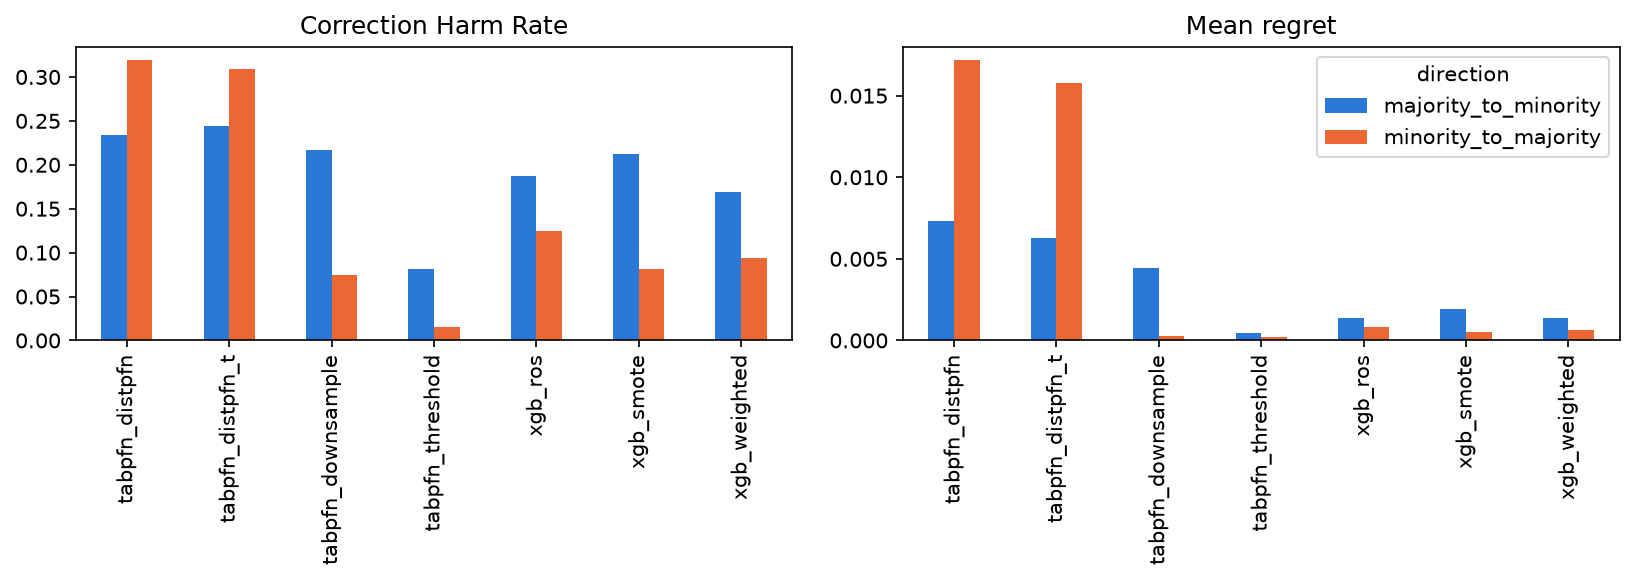
\includegraphics[width=0.85\linewidth]{figures/chr_regret.png}
\caption{Correction Harm Rate (left) and mean regret (right, $\max(0,-\text{CG})$)
by method and direction, over noisy stress cells only. \texttt{tabpfn\_distpfn}
has both a high CHR and the highest regret in both directions.
\texttt{tabpfn\_threshold} has the lowest of both in both directions.}
\label{fig:chr-regret}
\end{figure*}

Regret separates two methods that both have an elevated CHR under Direction
A, \texttt{tabpfn\_downsample} (21.7\%) and \texttt{tabpfn\_distpfn}
(23.4\%). Despite that similar failure frequency,
\texttt{tabpfn\_downsample}'s mean regret (0.0045) is well under
\texttt{tabpfn\_distpfn}'s (0.0073), and the gap widens sharply under
Direction B, where \texttt{tabpfn\_downsample}'s failure rate drops to
7.5\% while \texttt{tabpfn\_distpfn}'s rises to 31.9\%, and mean regret
moves from 0.0003 to 0.0172. When \texttt{tabpfn\_downsample} fails, it
tends to fail by a small margin regardless of direction.
\texttt{tabpfn\_distpfn}'s failures are both more frequent and, on average,
substantially larger.

Part of this asymmetry traces back to the uncorrected baselines themselves.
Comparing balanced accuracy at $c{=}0$ against $c{=}0.30$ for
\texttt{xgb\_none}, Direction B degrades performance by 0.079 (0.760 to
0.681) versus 0.032 for Direction A (0.760 to 0.729), roughly 2.5 times as
much. \texttt{tabpfn\_none} shows the same asymmetry, 0.067 (0.784 to 0.717)
versus 0.037 (0.784 to 0.747).
Losing genuine minority rows (Direction B) is inherently more damaging to
an uncorrected model than diluting the minority class with mislabeled
majority rows (Direction A), which helps explain why a correction's
apparent robustness under one direction does not predict its robustness
under the other.

\subsection{Break-Even Contamination Rates}
\label{sec:results-rq3}

Table~\ref{tab:breakeven} reports, for each method and direction, the share
of the 40 (dataset, $r$) combinations (30 for \texttt{tabpfn\_downsample}
under Direction A, since its 10 combinations at $r{=}0.50$ have no completed
runs to compute a break-even point from) whose seed-averaged Correction
Gain never dropped to zero or below within the tested range, i.e., $c^*>0.30$.
\texttt{tabpfn\_distpfn} remains the least likely of the seven to stay
beneficial across the full contamination range. It remains net-beneficial
through $c{=}0.30$ in only 35\% of conditions under Direction B, the lowest
share in the table, and 38\% under Direction A, tied with
\texttt{xgb\_smote} for the second-lowest. No single method leads at the
high end of the table. \texttt{tabpfn\_downsample} leads Direction A at
60\%, and \texttt{xgb\_smote} leads Direction B at 78\%.
\texttt{tabpfn\_threshold} stays beneficial through the full range in 70\%
of Direction B conditions, tied with \texttt{xgb\_ros} and
\texttt{xgb\_weighted} and trailing \texttt{xgb\_smote}, despite having by
far the lowest CHR and highest mean CG under that same direction. CHR
counts every failing cell individually, while break-even share only asks
whether a method's seed-averaged trend, aggregated within one (dataset,
$r$) combination, ever crosses zero. A method can have a low CHR and still
cross zero in many such combinations, which is exactly why
Section~\ref{sec:methods-contribution} defines CHR, Regret, and $c^*$ as
separate, complementary measures rather than collapsing robustness into one
number.

\begin{table}[t]
\centering
\caption{Share of (dataset, $r$) conditions where a method's seed-averaged
Correction Gain never dropped to zero or below within the tested
contamination range ($c^*>0.30$).}
\label{tab:breakeven}
\begin{tabular}{@{}lrr@{}}
\toprule
Method & Dir.\ A & Dir.\ B \\
\midrule
\texttt{xgb\_weighted}      & 48\% & 70\% \\
\texttt{xgb\_ros}           & 55\% & 70\% \\
\texttt{xgb\_smote}         & 38\% & 78\% \\
\texttt{tabpfn\_threshold}  & 55\% & 70\% \\
\texttt{tabpfn\_distpfn}    & 38\% & 35\% \\
\texttt{tabpfn\_distpfn\_t} & 40\% & 40\% \\
\texttt{tabpfn\_downsample} & 60\% & 70\% \\
\bottomrule
\end{tabular}
\end{table}

\subsection{Prior Sensitivity}
\label{sec:results-rq4}

The corrupted prior explains less of a correction's failure than expected.
On average, the deployable, observed-prior variant slightly outperforms
the oracle diagnostic rather than trailing it. Mean PSG
(Equation~\ref{eq:psg}) is negative for all three prior-dependent
methods in both directions. Under Direction A it is $-0.013$ for
\texttt{tabpfn\_threshold}, $-0.010$ for \texttt{tabpfn\_distpfn}, and
$-0.010$ for \texttt{tabpfn\_distpfn\_t}, with \texttt{tabpfn\_threshold}
the largest of the three in magnitude despite being the most robust method
on balanced accuracy. Under Direction B the gap is $-0.008$, $-0.020$, and
$-0.015$ respectively. This
gap is not fixed, however. Restricted to $c{=}0.30$ only, mean PSG for
\texttt{tabpfn\_distpfn} widens to $-0.042$ under Direction A, still the
widest of the three at that noise level, though the margin over
\texttt{tabpfn\_distpfn\_t} ($-0.041$) and \texttt{tabpfn\_threshold}
($-0.039$) is now narrow. Figure~\ref{fig:psg} shows the observed and
oracle curves for all three methods. At low contamination they stay close
together, but for the two DistPFN variants they separate sharply above
$c{=}0.20$ under Direction A, with the oracle variant degrading faster than
the observed one. \texttt{tabpfn\_threshold} shows the same ordering but a
much smaller gap. Even using the true, uncorrected prior does not fully
recover a correction's clean-condition performance once contamination is
severe. This means the corrupted prior is not the main reason these
corrections decline at high contamination.

\begin{figure*}[t]
\centering
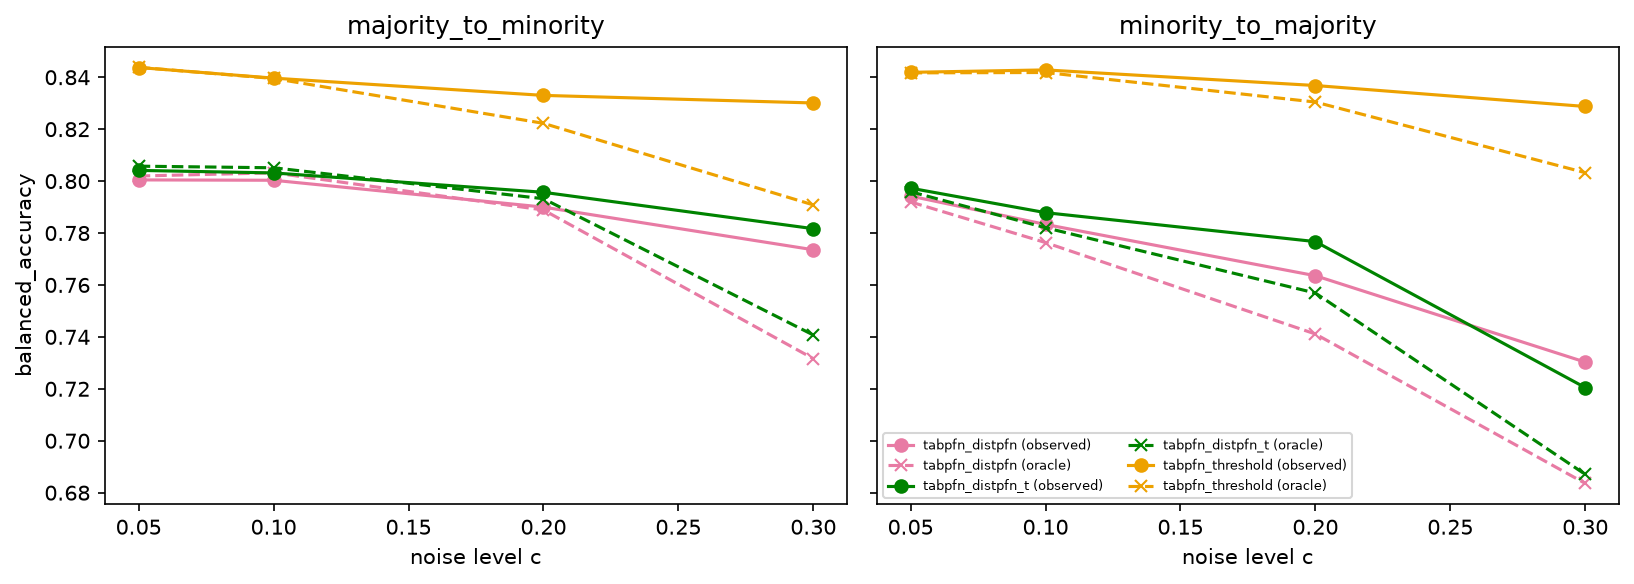
\includegraphics[width=0.85\linewidth]{figures/oracle_vs_observed.png}
\caption{Observed-prior (deployable, solid) versus oracle-prior (diagnostic,
dashed) balanced accuracy for the three prior-dependent TabPFN methods.
The oracle variant is never reliably better than the observed one, and for
\texttt{tabpfn\_distpfn} and \texttt{tabpfn\_distpfn\_t} it degrades faster
at high contamination under Direction A.}
\label{fig:psg}
\end{figure*}

\subsection{Statistical Significance}
\label{sec:results-significance}

Table~\ref{tab:friedman} reports the Friedman omnibus test for each model
family and corruption direction. All four are significant at $p<10^{-23}$,
so method identity significantly affects balanced accuracy within both
families in both directions.

\begin{table}[t]
\centering
\caption{Friedman omnibus test statistics by model family and corruption
direction. All four are significant at $p<10^{-23}$.}
\label{tab:friedman}
\begin{tabular}{@{}llrr@{}}
\toprule
Family & Direction & $\chi^2$ & $n$ (blocks) \\
\midrule
XGBoost & Dir.\ A & 111.1 & 160 \\
XGBoost & Dir.\ B & 198.9 & 160 \\
TabPFN  & Dir.\ A & 173.2 & 120 \\
TabPFN  & Dir.\ B & 332.7 & 160 \\
\bottomrule
\end{tabular}
\end{table}

Every uncorrected baseline differs significantly from every correction in
its family, in both directions (Holm-corrected $p<0.001$ throughout). The
corrections are having a measurable effect, even though
Section~\ref{sec:results-rq1} shows that effect is not always an
improvement.

Not every pair of corrections is distinguishable from each other, however.
\texttt{xgb\_weighted} and \texttt{xgb\_ros} are statistically
indistinguishable under Direction B ($p_{\text{Holm}}=0.95$). This is the
only non-significant pairwise comparison in the entire study. Every other
pairwise comparison, in both families and both directions, is statistically
significant.

\subsection{Calibration Reliability}
\label{sec:results-reliability}

Figure~\ref{fig:reliability} tracks Brier score and expected calibration
error against noise level for every method. Every XGBoost correction
improves on \texttt{xgb\_none}'s Brier score and ECE at every noise level
tested, in both directions, with no exception. The TabPFN family shows a
different kind of split. \texttt{tabpfn\_downsample} is worse-calibrated
than the uncorrected \texttt{tabpfn\_none} baseline on both metrics at
every noise level tested under Direction A, the only method in the study
with that pattern. \texttt{tabpfn\_threshold} never exceeds its baseline's
Brier score or ECE in either direction, which follows directly from how it
works: it only moves the decision threshold, so the underlying predicted
probabilities that Brier score and ECE measure are identical to
\texttt{tabpfn\_none}'s by construction. \texttt{tabpfn\_distpfn} and
\texttt{tabpfn\_distpfn\_t} do not merely avoid backfiring on calibration,
they are the two best-calibrated methods of any tested, correction or
baseline, at every noise level under Direction A and at every noise level
under Direction B except the highest tested, $c{=}0.30$, where
\texttt{tabpfn\_downsample} overtakes them on both metrics. This holds
despite the same two methods having the highest Correction Harm Rate in the
study on balanced accuracy (Section~\ref{sec:results-rq1}): a DistPFN
correction that frequently makes the wrong call can still be assigning that
call a well-calibrated probability, discrimination and calibration are not
the same failure mode. \texttt{tabpfn\_threshold} remains consistent with
its standing as the most robust method on balanced accuracy
(Sections~\ref{sec:results-rq1} and~\ref{sec:results-rq2}), but on raw
calibration it trails the two DistPFN variants throughout.

\begin{figure*}[t]
\centering
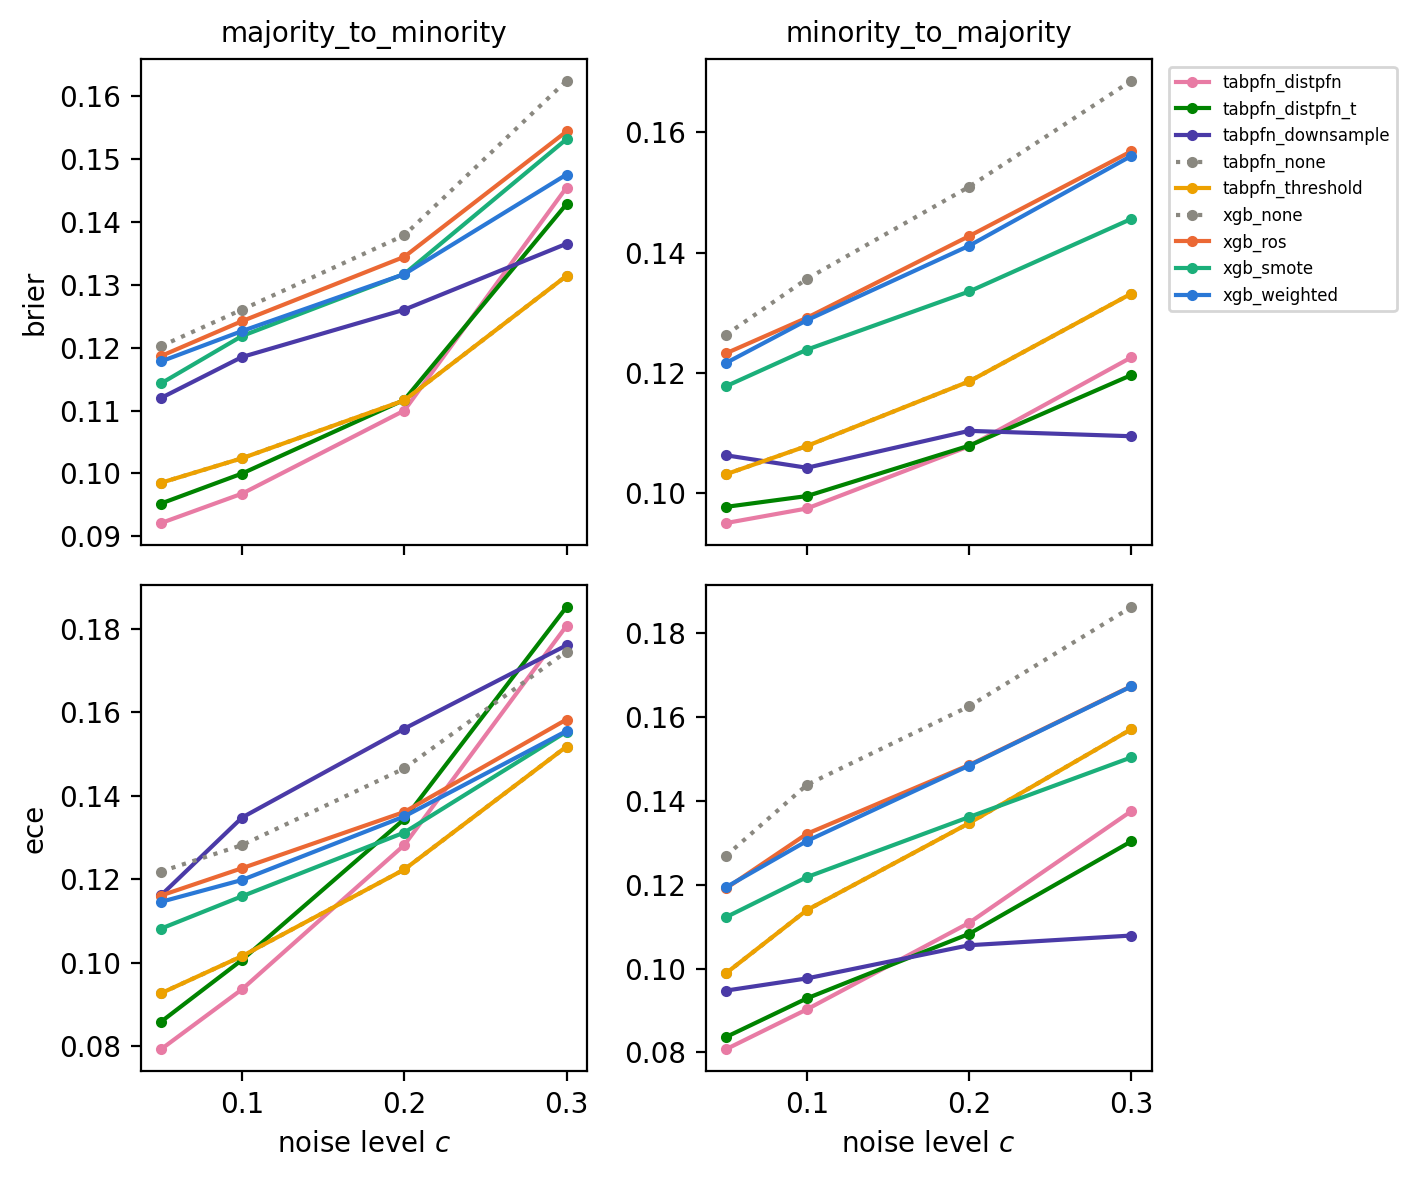
\includegraphics[width=0.85\linewidth]{figures/reliability.png}
\caption{Brier score (top) and expected calibration error (bottom) against
noise level, faceted by direction. Dotted gray lines are the two
uncorrected baselines. Every XGBoost correction improves on its baseline at
every noise level. Within the TabPFN family, \texttt{tabpfn\_downsample} is
the only correction that crosses above its own baseline, under Direction A,
while \texttt{tabpfn\_distpfn} and \texttt{tabpfn\_distpfn\_t} stay the
best-calibrated methods in the figure almost throughout.}
\label{fig:reliability}
\end{figure*}
